\chapter{Preliminares}
\label{cap-fundamentos} 
\section{Fundamentos}
    Este capítulo nos traz alguns conceitos básicos relativos à teoria dos grafos e convexidade que serão necessários ao longo dos demais capítulos.
Os conceitos e notações relativos à teoria dos grafos e algoritmos
estão baseados nas referências \cite{Bondy1976,Cormen2002}. Assim como as  definições, teoremas e resultados de convexidade também estão baseados nas referências 
\cite{Balogh,Barbosa2012,Bollobas,CeciliaCenteno2012,Centeno,Coelho2014,Coelho2012,duarte2015complexity,Hon2016,De2016a,Penso2015,DraquePenso2014}.

\subsection{Grafos e Convexidade}
    
Um \textit{grafo simples} $G$ é definido por um conjunto finito e não vazio de vértices $V(G)$ e um conjunto de arestas $E(G)$, formado por pares não ordenados de elementos de $V(G)$. Neste trabalho utilizaremos grafos simples finitos, em que arestas não formam laço com o próprio vértice de origem e mais de uma aresta ligando o mesmo par de vértice.

Na Figura~\ref{fig:grafo-exemplo} temos um exemplo de um grafo simples, 
com um conjunto $V(G)$ de seis vértices $V(G) = \{1, 2, 3, 4, 5, 6\}$, 
e um conjunto $E(G)$ de nove arestas $E(G) = \{(1,2), (1,5), (2,3), (2,5), (3,4), (3,5), (3,6), (4,5), (4,6)\}$.
Nota-se que não existe mais de uma aresta ligando o mesmo par de vértices e nenhuma aresta formando um laço. 

\begin{figure}
\centering
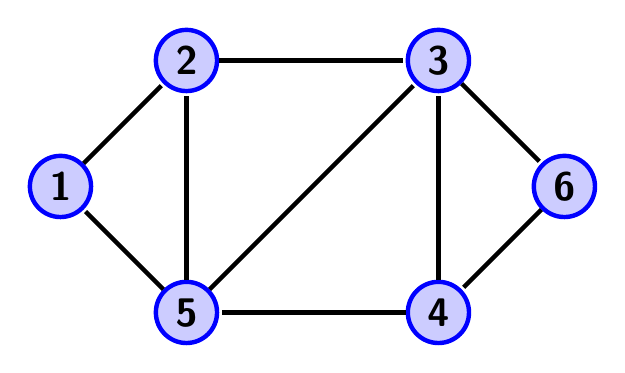
\begin{tikzpicture}[scale=0.8,shorten >=1pt, auto, node distance=3cm, ultra thick,
node_style/.style={circle,draw=blue,fill=blue!20!,font=\sffamily\Large\bfseries},
node_style_selected/.style={circle,draw=black,fill=red!20!,font=\sffamily\Large\bfseries},
edge_style/.style={draw=black}]
\node[node_style] (v1) at (-2,2) {2};
\node[node_style] (v2) at (2,2) {3};
\node[node_style] (v3) at (4,0) {6};
\node[node_style] (v4) at (2,-2) {4};
\node[node_style] (v5) at (-2,-2) {5};
\node[node_style] (v6) at (-4,0) {1};
\draw[edge_style]  (v1) edge node{} (v2);
\draw[edge_style]  (v2) edge node{} (v3);
\draw[edge_style]  (v3) edge node{} (v4);
\draw[edge_style]  (v4) edge node{} (v5);
\draw[edge_style]  (v5) edge node{} (v6);
\draw[edge_style]  (v6) edge node{} (v1);
\draw[edge_style]  (v5) edge node{} (v1);
\draw[edge_style]  (v5) edge node{} (v2);
\draw[edge_style]  (v4) edge node{} (v2);
\end{tikzpicture}
\caption{Exemplo de um grafo}
\label{fig:grafo-exemplo}
\end{figure}


A \textit{vizinhança aberta} de um vértice consiste no conjunto de todos os seu vizinhos, e será denotada por: seja $v$ um vértice de $G$ então sua vizinhança aberta é $N_G(v)=N(v)=\{u \in V(G)|vu \in E(G)\}$. Ao passo que dado um conjunto qualquer de vértices a \textit{vizinhança aberta de um conjunto} é a união da vizinhança aberta de todos os seus elementos, denotada por $N_G(S)=N(S)=\{\forall v \in S| u \in N(S)|vu \in E(G)\}$.  A \textit{vizinhança fechada} é o conjunto formado pela vizinhança aberta do vértice união com ele próprio, será dada por $N_G[v] = N[v]=\{v\} \cup N_G(v)$. De maneira análoga  a \textit{vizinhança fechada de um conjunto}, consiste na união da vizinhança fechada de todos os seus elementos, denotada por $N_G[S]=N[S]=S\cup N(S)$.

Seja um grafo qualquer $G$, um \textit{subgrafo} de $G$ é um grafo $H$ cujo conjunto de vértices seja um subconjunto de $V(G)$ e o conjunto de arestas é um subconjunto de $E(G)$. Dado um subconjunto $S$ de vértices de $G$, podemos dizer que um \textit{subgrafo induzido}, é um subgrafo cujo conjunto de vértices é $S$, e o conjunto de arestas é o subconjunto de todas as arestas de $G$ que tenham as duas extremidades $S$. Dado um grafo $G$ e um vértice $v$ tal que $v \in V(G)$, para facilidades de notação, o subgrafo $G'$ induzido pelo conjunto de vértice $V(G)\setminus\{v\}$, será representado como $G'=G-v$.

Um \textit{caminho} em $G$ é uma sequência de vértices $P=v_0,v_1,\cdots,v_k$, tal que $v_iv_{i+1} \in E(G)$ para $i$ de $0$ até $k-1$. A \textit{distância} entre dois vértices é o comprimento do menor caminho entre eles. Sejam $u$ e $v$ dois vértices distintos de um grafo $G$. Vamos denotar a distância entre eles como $d_G(u,v)=d(u,v)$. E o \textit{diâmetro} de $G$ é a maior distância entre quaisquer dois vértices, será dado por $diam(G)=d$. 

Um grafo $G$ é dito \textit{conexo}, se para todo par de vértice existe um caminho de um para o outro. Caso contrário ele é tido como \textit{desconexo}. Em um grafo desconexo uma \textit{componente conexa} é formada por um conjunto de vértices que possuem caminho entre si, ou seja todos os vértices de uma componente conexa são acessíveis a outros vértices na mesma componente. O número de componentes conexas de $G$ será denotado por $\omega(G)$. Um grafo $G$ possui um \textit{vértice de corte} $c$ se o subgrafo $G'= G-c$ e tal que $\omega(G^\prime)>\omega(G)$. Por fim $G$ é dito \textit{biconexo} se é conexo e não possui vértice de corte. 

O \textit{grau}  de um vértice $v$ de $G$, será denotado como $d_G(v)=d(v)$ e é o número de arestas incidentes em $v$. O maior e menor graus dos vértices de $G$ serão respectivamente denotados por $\delta(G)$ e $\Delta(G)$. 

Um subconjunto $D \subseteq V(G)$ é um \textit{conjunto dominante} de $G$, se para todo $v \in V(G) \setminus D$, $v$ é adjacente a pelo menos um vértice de $D$. Um subconjunto $D \subseteq V(G)$ é um \textit{conjunto dominante total} de $G$, se para todo $v \in V(G)$, $v$ é adjacente a pelo menos um vértice de $D$.  A \textit{cintura} de um grafo $G$ é o menor ciclo de $G$. Um grafo $G((A,B),E)$ é dito \textit{bipartido} se seus vértices podem ser particionados em dois subconjuntos $A$ e $B$, de forma com que toda aresta de $G$ tem um extremo em $A$ e outro em $B$. $G$ é um grafo \textit{bipartido completo} se todo vértice em $A$ é adjacente a todo vértice em $B$. Por fim, $G$ é $k-$partido se os vértices de $G$ puderem ser particionados em $k$ subconjuntos, de forma que os vértices pertencentes a mesma partição não sejam adjacentes.

Um subconjunto $C_t \subseteq V(G)$ é um \textit{corte de vértices}, se a remoção de todos os vértices em $C_t$ desconecta $G$, de forma análoga com as arestas, um subconjunto $C_t \subseteq E(G)$ é um \textit{corte de arestas} se a remoção de todas as arestas desconecta $G$. Um \textit{corte mínimo} em um grafo é um subconjunto de vértices ou arestas, tal que não existe um subconjunto menor que é um \textit{corte de vértices} ou \textit{corte de arestas}, respectivamente.

Os grafos $G_1$ e $G_2$, são considerados \textit{isomorfos} se existe uma função $f$ bijetora tal que $f: V(G_1) \to V(G_2)$ e $u,v\in E(G_1)$ se somente se $f(u),f(v) \in E(G_2)$. Considerando essa relação como \textit{isomorfismo} temos o \textit{automorfismo} que é um isomorfismo de um grafo consigo mesmo, ou seja, em um grafo $G$ existem permutações de seus vértices, que são isomorfismos de $G$. Ainda no campo do \textit{automorfismo} para quaisquer dois pares de vértices de um grafo $G$, existe um automorfismo, então temos $G$ que é um grafo \textit{vértice-transitivo}, e se para qualquer dois pares de vértices a uma distância determinada, existe um automorfismo para qualquer outros dois pares de vértices a mesma distância, então $G$ é um grafo \textit{distância-transitivo}.


São tipos especiais de grafos, usados como exemplo mais a frente. O \textit{grafo estrela} é um grafo bipartido completo em que uma partição possui somente um vértice, em um \textit{grafo completo} todo par de vértice é adjacente entre si, um \textit{grafo caminho} consiste em um grafo conexo conexo, com dois ou mais vértices, que podem ser ordenados em um caminho passando por todos seus vértices, e por ultimo o \textit{grafo ciclo} que é um grafo que contem um único ciclo composto por todo os sues vértices. 


De modo geral, uma \textit{convexidade} em um grafo $G$ é dada por um conjunto ${\cal C}$, formado por subconjuntos de V(G) que atende as seguintes restrições:
\begin{itemize}
    \item[-] $\emptyset,V(G) \in {\cal C}$;
    \item[-] ${\cal C}$ é um conjunto fechado em relação a operação de interseção.
\end{itemize}
    Cada elemento de ${\cal C}$ é um \textit{conjunto convexo}
para uma convexidade ${\cal C}$. A \textit{envoltória convexa} $H_c(S)$ 
de um subconjunto $S$ é o menor conjunto convexo que contém S.
Um tipo de convexidade especial em grafos são as convexidades definidas através de um conjunto
${\cal P}$ de caminhos em grafos. Neste caso, um subconjunto ${\cal C} \in V(G)$ é convexo, principalmente
quando ${\cal C}$ contém todos os vértices pertencentes aos caminhos de ${\cal P}$ cujos vértices extremos estão também em ${\cal C}$. 

Podemos citar a \textit{convexidade geodésica},
definida no momento em que ${\cal P}$ é o conjunto de todos os caminhos mínimos de G, 
veja em \cite{Caceres2006,Dourado2016,Journal2010}, e também a \textit{convexidade $P_3$},
quando ${\cal P}$ é o conjunto de todos os caminhos com três vértices 
\cite{Barbosa2012,Centeno,Centeno2011,Coelho2014,Dourado2013}.

\subsection{Convexidade $P_3$}
\label{sec-convexidade-p3}
    De agora em diante iremos considerar ${\cal C}$ como convexidade $P_3$.
Como um grafo $G$ unicamente determina sua convexidade $P_3$ utilizaremos
$H(S)$ ao invés de $H_c(S)$.

Dado um subconjunto $S \subseteq V(G)$, o \textit{intervalo fechado} 
$I{[}S{]}$ de $S$ é formado por $S$ simultaneamente com todo vértice de $V(G) \setminus S$
com pelo menos dois vizinhos em $S$. Se $I{[}S{]}=S$ então $S$ é um conjunto convexo.
Podemos utilizar o intervalo fechado para iterativamente calcular a envoltória convexa de 
um subconjunto $S \subseteq V(G)$. Assim a envoltória convexa pode ser formada
por uma sequência $I^p[S]$ onde $p$ é um inteiro não negativo,  
$I^0{[}S{]}=S$, $I^1{[}S{]}=I{[}S{]}$ e $I^p{[}S{]}=I[I^{p-1}]$ para $p \ge 2$.
Quando para algum $p$, temos $I^q{[}S{]} = I^p{[}S{]}$, para todo $q \ge p$, temos
então $I^p{[}S{]}$, considerando-o  um conjunto convexo.

Considere o grafo $G$ na Figura~\ref{fig:grafo-petersen} e o subconjunto $S_0 = \{4, 5, 8, 9\}$ de V(G). O Conjunto $S_0$ não é um conjunto convexo, por exemplo, existe o caminho $P=5,7,9$ em que os vértices $5$ e $9$ então no conjunto e o vértice $7$, vizinho a $5$ e $9$, não está. Já que o conjunto não é convexo, qual seria o menor conjunto convexo que contém $S_0$?
Para responder essa pergunta, precisamos calcular a envoltória convexa de $S_0$, 
tal como se segue:

Vamos computar a envoltória convexa do conjunto $S_0$:
\begin{itemize}
    \item{$I^1{[}S_0{]}=\{0, 3, 4, 5, 6, 7, 8, 9\}$}
    \item{$I^2{[}S_0{]}=I{[}I^1{[}S_0{]}{]}=\{0, 1, 2, 3, 4, 5, 6, 7, 8, 9\}$}
    \item{$I^3{[}S_0{]}=I{[}I^2{[}S_0{]}{]}=I^2{[}S_0{]}=\{0, 1, 2, 3, 4, 5, 6, 7, 8, 9\}$}
\end{itemize}

    Com isso determinamos o menor conjunto convexo para o grafo do exemplo 
que contém o conjunto $S_0$. Logo $H(S_0)=\{0, 1, 2, 3, 4, 5, 6, 7, 8, 9\}$.

\begin{figure}
\centering
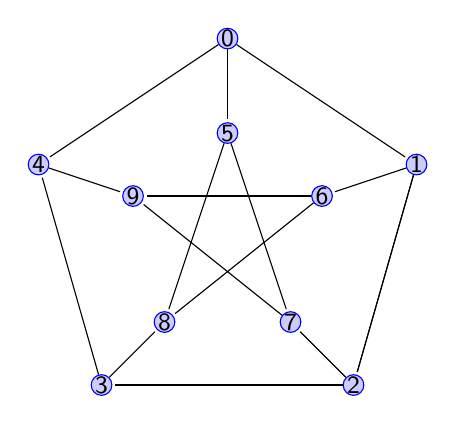
\begin{tikzpicture}[scale=0.8,shorten >=1pt, auto, node distance=3cm,
node_style/.style={circle,draw=blue,fill=blue!20!,inner sep=0pt, minimum width=4pt,font=\sffamily\small},
node_style_selected/.style={circle,draw=black,fill=red!20!,font=\sffamily\Large\bfseries},
edge_style/.style={draw=black}]
\node[node_style] (v0) at (0,3.5) {0};
\node[node_style] (v1) at (3,1.5) {1};
\node[node_style] (v2) at (2,-2) {2};
\node[node_style] (v3) at (-2,-2) {3};
\node[node_style] (v4) at (-3,1.5) {4};
\node[node_style] (v5) at (0,2) {5};
\node[node_style] (v6) at (1.5,1) {6};
\node[node_style] (v7) at (1,-1) {7};
\node[node_style] (v8) at (-1,-1) {8};
\node[node_style] (v9) at (-1.5,1) {9};

\draw[edge_style]  (v0) edge node{} (v1);
\draw[edge_style]  (v0) edge node{} (v4);
\draw[edge_style]  (v0) edge node{} (v5);
\draw[edge_style]  (v1) edge node{} (v2);
\draw[edge_style]  (v1) edge node{} (v2);
\draw[edge_style]  (v1) edge node{} (v6);
\draw[edge_style]  (v2) edge node{} (v3);
\draw[edge_style]  (v2) edge node{} (v7);
\draw[edge_style]  (v3) edge node{} (v4);
\draw[edge_style]  (v3) edge node{} (v8);
\draw[edge_style]  (v4) edge node{} (v9);
\draw[edge_style]  (v5) edge node{} (v7);
\draw[edge_style]  (v5) edge node{} (v8);
\draw[edge_style]  (v6) edge node{} (v8);
\draw[edge_style]  (v6) edge node{} (v9);
\draw[edge_style]  (v7) edge node{} (v9);
\end{tikzpicture}
\caption{Grafo de Petersen, $G_{pn}$}
\label{fig:grafo-petersen}
\end{figure}

Se $H(S)=V(G)$ dizemos que $S$ é  um \textit{conjunto de envoltória}, ou conjunto envoltório. 
A cardinalidade $h(G)$ do menor conjunto de envoltória em $G$ é chamado de 
\textit{número envoltório}.

Apesar da aparente simplicidade proveniente da definição,
os estudos em \cite{Dourado2009} permitem inferir que determinar o número envoltório para grafos gerais é um prolema NP-Completo.

No exemplo da Figura~\ref{fig:grafo-petersen} 
temos a envoltória convexa do conjunto $S_0$ que é equivalente ao conjunto de vértices.
Nesse caso, temos que $S_0$ é um conjunto de envoltória, porém, existem conjuntos de envoltória de cardinalidade menor que $S_0$,
como por exemplo $S_1=\{4,7,8\}$. Como não existe nenhum conjunto de envoltória de cardinalidade 2, concluímos que h(G)=3.


Um resultado habitual sobre os conjuntos convexos no ${\cal R}^d$ é o teorema de Carathéodory \cite{Caratheodory1911}.
Este teorema afirma que todo ponto $u$ na envoltória convexa de um conjunto $S \subseteq {\cal R}^d$ encontra-se no fecho
convexo de um subconjunto $F$ de $S$ de ordem no máximo $d+1$. Do teorema de Carathéodory surge  a definição do número de 
Carathéodory para grafos. Seja $G$ um grafo e ${\cal C}$ uma convexidade sobre V(G).
O \textit{número de Carathéodory} c(G) é o menor inteiro c,
para o qual todo $u \in H(S)$, existe um conjunto $F \subseteq  S$,
com $|F| \le c$ e $u \in H(F)$. 

Seja $G$ um grafo e $S$ um subconjunto de V(G). Se $\partial H(S)=H(S) \setminus \bigcup _{u \in S} H(S \setminus \{u\})$,
é não vazio, então $S$ é um \textit{conjunto de Carathéodory}. Esta definição permite um sistema alternativa,
o número de Carathéodory como sendo a maior cardinalidade de um conjunto de Carathéodory. 

Considere o grafo $G$ da Figura~\ref{fig:grafo-petersen}. Observe que $S_1=\{4,7,8\}$ é um conjunto de 
Carathéodory, porém, existem conjuntos de Carathéodory de cardinalidade maior que $S_1$, como por exemplo o
próprio conjunto $S_0 = \{4,5,8,9\}$. Note que $H(S_0)=\{0, 1, 2, 3, 4, 5, 6, 7, 8, 9\}$.
Neste momento aplicando a definição do conjunto de Carathéodory iremos determinar o $\partial H(S_0)$:
\begin{itemize}
    \item{Conforme já determinado anteriormente, $H(S_0)=\{0, 1, 2, 3, 4, 5, 6, 7, 8, 9\}$}
    \item{Aplicando a envoltória convexa, temos $H(S_0 \setminus \{4\})=\{5,8,9,6,7\}$}
    \item{Aplicando a envoltória convexa, temos $H(S_0 \setminus \{5\})=\{4,8,9,3,6\}$}
    \item{Aplicando a envoltória convexa, temos $H(S_0 \setminus \{8\})=\{4,5,9,0,7\}$}
    \item{Aplicando a envoltória convexa, temos $H(S_0 \setminus \{9\})=\{4,5,8,0,3\}$}
    %\item{Aplicando a envoltória convexa, temos $H(S_0 \setminus \{9\})=\{4,5,8,0,3\}$}
    \item{$\partial H(S_0)=H(S_0) \setminus (H(S_0 \setminus \{4\}) \cup H(S_0 \setminus \{5\}) \cup H(S_0 \setminus \{8\}) \cup H(S_0 \setminus \{9\}))$}
    \item{Com os resultados anteriores podemos obter a informação de que: $\partial H(S_0)=\{1,2\}$}
\end{itemize}

Como o conjunto $\partial H(S_0)$ não é vazio, 
podemos concluir que $S_0$ é um conjunto de Carathéodory.
Dado que não existem conjuntos de Carathéodory 
de cardinalidade maior do que quatro,
alimentamos que esse é o número de Carathéodory do grafo $G$,
isto é, $c(G_{pn})=4$.

Em \cite{Barbosa2012} demonstra-se que determinar o Número de Carathéodory na Convexidade $P_3$
é um problema NP-Completo mesmo para grafos bipartidos. 
Podemos inferir assim, a dificuldade na definição de tal parâmetro para grafos gerais. 
Embora o problema seja NP-Completo, 
para algumas classes foi possível definir um limite máximo 
ou um algoritmo polinomial que determine esse parâmetro,
tais como árvores e blocos \cite{Coelho2012}. 


\subsection{Algoritmos e Classe de Complexidade}

Três classes de problema são bem conhecidas na literatura: P, NP e NP-Completo. 
A classe P trata-se da classe dos problemas com solução polinomial, isto é, problemas que admitem algoritmos em tempo $O(n^c)$ em que $c$ é uma constante e $n$ o tamanho da entrada.
São na prática, problemas tido como tratáveis. A segunda classe, 
os problemas NP, são os problemas cujo certificado da solução pode ser verificado em tempo polinomial.

Por fim, temos a classe de problemas NP-Completo,
que consistem em problemas NP e cuja complexidade 
é igual ou superior aos problemas mais difíceis em NP.
Até o momento, não é conhecido solução polinomial para qualquer problema dessa classe. Por isso os problemas nessa classe, são tidos na prática como 
computacionalmente intratáveis.

Uma interessante subclasse dos problemas NP-Completo,
são os Pseudo-polinomiais ou Quasi-polinomiais.
Diz respeito a problemas que para determinadas instâncias de problemas
tem complexidade polinomial para determinados parâmetros da entrada.
Por exemplo, sabemos que é um problema NP-Completo determinar se um grafo $G$, com $n$ vértices, tem um conjunto envoltório de tamanho $k$. Mas, se para certas classes de grafos, for possível encontrar um conjunto envoltório em tempo polinomial, quando $k$ maior que uma função determinada $k>f(n)$, podemos dizer que o número envoltório é um problema pseudo-polinomial quando restrito as classes específicas.


%Nesse caso temos que como entrada do problema o grafo e a constante $k$, mas podemos determinar que para certas classes de grafos, se conseguirmos determinar que é possível encontrar um conjunto envoltório em tempo polinomial, quando for $k$ maior que uma função determinada $k>f(n)$, podemos dizer que o número envoltório é um problema pseudo-polinomial nesses casos. 

%Os problemas NP-Completos remanescem na literatura como intratáveis.
%Até o momento não foi possível demonstrar que admitem solução polinomial
%ou mesmo que é impossível.

Segundo \cite{Cormen2002} muitos problemas NP-Completos,
apesar de intratáveis, são relevantes demais para não se tentar uma solução. 
De acordo com \cite{Cormen2002} há três possíveis caminhos:
1) O isolamento de casos específicos e que possam ser resolvidos polinomialmente;
2) Um algoritmo exponencial para entradas relativamente pequenas;
3) Algoritmos heurísticos que produzam soluções quase ótimas.

Neste trabalho, exploramos um pouco de cada um desses caminhos
para obter um conjunto de soluções capazes de auxiliar 
nos estudos dos parâmetros de convexidade $P_3$.

Existem casos polinomiais identificados na literatura
que foram listados na revisão bibliográfica. 
No resultado das execuções outros possíveis casos foram identificados
e serão mencionados no que se refere aos resultados obtidos.

Para que entradas mais avançadas pudessem ser analisadas
os algoritmos exponenciais foram implementadas em duas versões, uma sequencial e outra paralela. 
Na implementação paralela foi utilizada a arquitetura CUDA,
que é baseada nas Unidades de Processamento Gráfico (GPU) da NVIDIA.
Pois ela nos permite o uso deste poder de processamento de baixo custo para computação de propósito geral.

A programação paralela eficiente traz vários desafios ausentes na programação tradicional, 
tais como: - equilibrar de maneira mais igualitária possível o trabalho das \textit{threads}, - utilizar o mínimo necessário de acesso a memória global e a sincronização de \textit{threads}, -uniformizar o acesso aos dados de trabalho das \textit{threads} o máximo possível,
dentre outros, sob pena da solução paralela ser mais ineficiente do que a solução sequencial.

Os algoritmos heurísticos foram concebidos a partir de uma abordagem gulosa,
onde em cada etapa a melhor solução é escolhida localmente na 
tentativa de maximizar ou minimizar o resultado final. 
Apesar de ser uma abordagem simples para tratar de um problema NP-Completo,
apresentou bons resultados para alguns tipos de grafos.

%/* Explicação breve sobre complexidade de algoritmo, força bruto e algoritmos aproximativos */


\section{Grafos de diâmetro 2}

Um grafo $G$ é dito de diâmetro 2 se a maior distância entre quaisquer dois vértices é 2. Em outras palavras, $G$  não é completo e todo par de vértices $u,v \in V(G)| (u,v) \in E(G)$ ou $N(u) \cap N(v) \ne \emptyset$. A classe de grafos de diâmetro 2 é ampla e inclui duas classes de interesse desse trabalho: é fortemente Regular conexos e Maximais Sem triângulo, cujo as definições já foram apresentadas anteriormente.

Apesar de serem classes distintas, existem alguns grafos fortemente regulares que também são maximais sem triângulo.  Esses grafos são também conhecidos como \textit{fortemente regulares sem triângulo}, que podemos ver na Figura~\ref{figconjts}. Na literatura atual são conhecidos apenas sete: $C_5$, grafo de Petersen, Clebsch, Hoffman-Singleton, Gewirtz e Higman-Sims. Ainda subsiste desconhecido um oitavo grafo de diâmetro 2 e fortemente regular, que caso venha se confirmar poderemos dizer que é um grafo de Moore 57-regular, contendo 3250 vértices e cintura 5 \cite{Godsil1995}.

\begin{figure}[h]
    \centering
    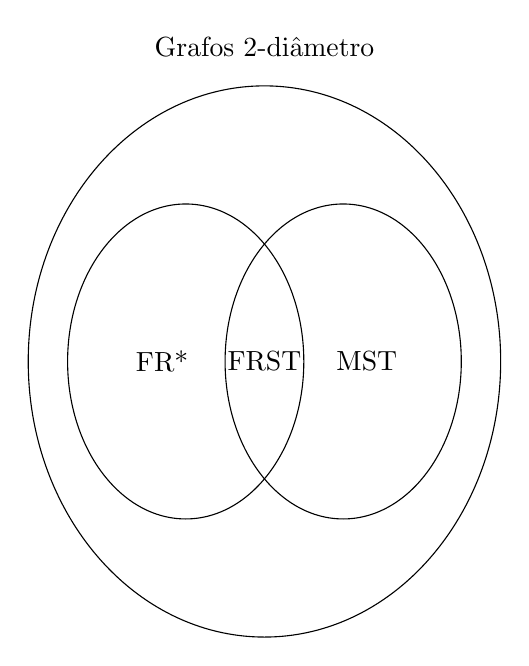
\begin{tikzpicture}
    \draw  (-2,2) ellipse (1.5 and 2);
    \draw  (0,2) ellipse (1.5 and 2);
    \draw  (-1,2) ellipse (3 and 3.5);
    \node at (-1,2) {FRST};
    \node at (-1,6) {Grafos 2-diâmetro};
    \node at (-2.3,2) {FR*};
    \node at (0.3,2) {MST};
    \end{tikzpicture}
    \caption{Grafos de 2-diâmetro, Fortemente Regular Conexos (FR*), Maximais Sem Triângulo (MST) e Fortemente Regulares Sem Triângulo (FRST)}
    \label{figconjts}
\end{figure}

\subsection{Maximal Sem Triângulo}
\label{sec-mst}
Um grafo $G$ é \textit{maximal sem triângulo} se a adição de qualquer aresta em $G$
formar um triângulo. Um grafo $G$ é dito \textit{diâmetro 2-crítico} ou \textit{diâmetro 2 minimal}  se ele tem diâmetro 2 e a remoção de qualquer aresta implica em um aumento do diâmetro do grafo. Em outras palavras $G$ é \textit{diâmetro 2-crítico} se $d(G)=2$ e $\forall e\in E(G) \Rightarrow d(G-e)>2$.  Em \cite{Mathematics1995,Barefoot1995} temos a demonstração  de que todo grafo maximal sem triângulo é um grafo de diâmetro 2 minimal, cuja deleção de qualquer aresta aumentaria o diâmetro do grafo. Enquanto para \cite{Brandt2000} todo grafo com pelo menos 3 vértices e diâmetro 2 é um grafo livre de triângulo. Exemplos: grafo estrela, completo bipartido e grafo de Petersen. 


 %Theorem 1: A triangle-free Graph is MTF if and only if it is MD2. [BAREFOOT199593]
%Não econtrei definição melhor em artios em inglês é referenciado como "diameter 2-critical graphs",
% porém não encontrei nenhum bom artigo em português que os cite


\subsection{Fortemente regular}
\label{sec-fr}

Um grafo $G$ é \textit{fortemente regular} se for um grafo k-regular 
e existir dois inteiros $b$ e $c$ tais que todos dois vértices adjacentes têm $b$ vizinhos em comum e todos dois vértices não adjacentes têm $c$ vizinhos em comum, podendo ser definido pelos parâmetros $(n,k,b,c)$. Tais como exemplos, temos alguns grafos bastante conhecidos e seus respectivos parâmetros listados na Tabela~\ref{tab-exemplos-grafos-fr}.
%Octahedral (6,4,2,4), $C_5$ (5,2,0,1), Hoffman-Singleton (50,7,0,1), Gewirtz (56,10,0,2) e Berlekamp-van Lint-Seidel (243,22,1,2). Se o parâmetro $c=0$ então o grafo é desconexo ou completo, pois todo par de vértice não é adjacente ou não possui vizinhos em comum. Os grafos fortemente regulares desconexos não são objeto de estudo deste trabalho.

\begin{table}[h]
\centering
\caption{Exemplos de grafos e parâmetros}
\label{tab-exemplos-grafos-fr}
\begin{tabular}{|l|l|}
\hline
\textbf{Grafo}            & \textbf{Parâmetro} \\ \hline
Octahedral                & (6,4,2,4)          \\ \hline
$C_5$                     & (5,2,0,1)          \\ \hline
Hoffman-Singleton         & (50,7,0,1)         \\ \hline
Gewirtz                   & (56,10,0,2)        \\ \hline
Berlekamp-van Lint-Seidel & (243,22,1,2)       \\ \hline
\end{tabular}
\end{table}

%/* Aparentemente é um probLema em aberto na literatura a quantidade desses grafos,
% 7  sãoconhecidos: http://www.math.ru.nl/OpenGraphProblems/Tjapko/30.html 
%Artigo Norman Brigs (não publicado): https://arxiv.org/pdf/0911.2160.pdf %http://www.maths.lse.ac.uk/Personal/norman/SRNT.pdf
%*/



\subsection{Propriedades dos Grafos de diâmetro 2}

Os grafos de diâmetro 2 possuem importantes propriedades. Podemos citar a cintura $g$ que é $3 \le g \le 5$, ou infinita quando é uma estrela \cite{Desormeaux2013}. Outra propriedade importante é que para qualquer $v \in V(G)$ o conjunto $N(v)$ é um conjunto dominante, ou seja, o conjunto formado pelos vizinhos de qualquer vértice é um conjunto dominante, conforme ilustrado na Figura~\ref{fig:tds}.

\begin{figure}
\centering
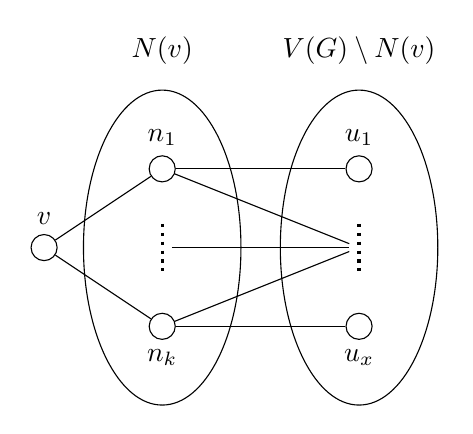
\begin{tikzpicture}
    \draw  (0,0) ellipse (1 and 2);
    \node[circle,draw,label=$v$] (v1) at (-1.5,0) {};
    \node[circle,draw,label=$n_{1}$] (v2) at (0,1) {};
    \node[circle,draw,label=below:$n_{k}$] (v3) at (0,-1) {};
    \draw [very thick,dotted] (0,0.3) -- (0,-0.3);

    \node (v7) at (0,0) {};

    \draw  (v1) edge (v2);
    \draw  (v1) edge (v3);

    \node at (0,2.5) {$N(v)$};

    \draw  (2.5,0) ellipse (1 and 2);
    \node at (2.5,2.5) {$V(G) \setminus N(v)$};

    \node[circle,draw,label=$u_1$] (v4) at (2.5,1) {};
    \node (v5) at (2.5,0) {};
    \draw [very thick,dotted] (2.5,0.3) -- (2.5,-0.3);
    \node[circle,draw,label=below:$u_x$] (v6) at (2.5,-1) {};

    \draw  (v2) edge (v5);
    \draw  (v2) edge (v4);
    \draw  (v3) edge (v6);
    \draw  (v3) edge (v5);
    \draw  (v7) edge (v5);
\end{tikzpicture}
\caption{$\forall v \in V(G)$  $N(v)$ é um conjunto dominante}
\label{fig:tds}
\end{figure}

\begin{proposition} Seja G um grafo de diâmetro 2.
\begin{enumerate}[label=(\alph*)] % (a), (b), (c), ...
   \label{prop:diametro2}
    \item{Para todo $u,v \in V(G)$, $u$ e $v$ são adjacentes ou tem um vizinho em comum} \label{pro-diam-2-itema}
    \item{$N(v)$ é um conjunto dominante $\forall v \in V(G)$} \label{pro-diam-2-itemb}
    \item{Se $\delta(G)=1$ então $\Delta(G)=n-1$}
    \item Se $v \in V(G)$ é um vértice de corte então $d(v)=n-1$\label{pro-diam-2-itemd}
    \item{Se $G$ tem vértice de corte então $\Delta(G)=n-1$}\label{pro-diam-2-iteme}
    \item Existe no máximo um vértice de corte em $G$\label{pro-diam-2-itemf}
    \item{Se $v_1,v_2 \in V(G)$ então $N[v_1] \cap N[v_2] \ne \emptyset$}
\end{enumerate}
\end{proposition}
\begin{proof}

Se $G$ tem diâmetro 2, então qualquer vértice $u$ tem um caminho até outro vértice $v$ passando por no máximo 2 arestas. Desta forma todo par de vértice em $G$ é adjacente ou possuem um vértice em comum, podemos assim concluir a proposição ~\ref{prop:diametro2}(a).

$N(v)$ é um conjunto dominante. Seja $u$ e $v$, dois vértices não adjacentes, supomos por contradição que não existe aresta de $u$ param $N(v)$, então não existe caminho $vwu$ visto que $w\in N(v)$, dessa forma a menor distância de $u,v$ é maior do que dois o que é uma contradição, pois $G$ tem diâmetro 2. Dessa forma podemos concluir a proposição ~\ref{prop:diametro2}(b).

Se $\delta(G)=1$ então $\exists v \in V(G)|d(v)=1$. Pela proposição anterior $N(v)$ é um conjunto dominante, como $v$ possui um único vizinho $u$, então $u$ é adjacente a todos os vértices $V(G)\setminus \{u\}$, e $d(u)=|V(G)|-1=n-1$. Com isso temos provado a proposição ~\ref{prop:diametro2}(c).

Se $G$ possui um vértice de corte $c$ e $\omega(G-c)$ o número de componentes conexas de $G-c$, então $\omega(G-c)>1$. Seja $C_x$ as componentes conexas do grafo $G-c$, supomos por contradição que $d(c)<n-1$, então existe um vértice $v \in C_i$, que não é adjacente a $c$ e nenhum vértice em $C_j$, tal que $i\neq j$. Porém, como $G$ tem diâmetro 2 então $\forall u \in C_j$, existe um caminho $uwv$ tal que $w\ne c$, dessa forma $v$ é adjacente a todos os vértices de $C_j$, o que consideramos uma contradição, pois, estão em componentes conexas distintas. Isso prova ~\ref{prop:diametro2}(d).

Se $G$ possui um vértice de corte, pela Proposição~\ref{pro-diam-2-itemd}, existe um vértice $v$ tal que $d(v)=n-1$. Por $G$ ser um grafo simples então não existe vértice $u\in V(G)$ tal que $d(u)>d(v)=n-1$. Portanto, concluímos que $\Delta (G) = n-1$. Isso prova ~\ref{prop:diametro2}(e).

Supomos por contradição que $G$ possui dois ou mais vértices de corte, $v_1,v_2,...,v_k$. Pela Proposição~\ref{pro-diam-2-itemd} sabemos que esses vértices são adjacentes a todos os demais vértices de $G$, então temos o grafo $G-v_1$ que possui duas ou mais componentes conexas. Em uma das componentes conexas teremos $v_2$ que também é um vértice de corte, em outra componente conexa distinta teremos $v_c$, por $v_2$ ser um vértice de corte é adjacente a todos os demais vértices inclusive $v_c$. Portanto, deveriam estar na mesma componente conexa, o que é uma contradição, pois, $v_c$ pertence a uma componente conexa diferente de $v_2$, logo, concluímos que $\Delta (G) = n-1$, o que prova ~\ref{prop:diametro2}(f).

Seja $G$ um grafo de diâmetro 2 e vértices $v_1,v_2 \in V(G)$ então $N[v_1] \cap N[v_2] \ne \emptyset$. Se $v_1$ e $v_2$ são adjacentes então $\{v_1, v_2\} \subseteq N[v_1] \cap N[v_2]$. Se $v_1$ e $v_2$ não são adjacentes, então por definição $\exists n_1 \in V(G)$ tal que $n_1 \in N(v_1) \cap N(v_2)$, o que implica na proposição ~\ref{prop:diametro2}(g) e que pode ser visto na Figura~\ref{fig:setunion}.
\end{proof}

\begin{figure}[h]
\centering
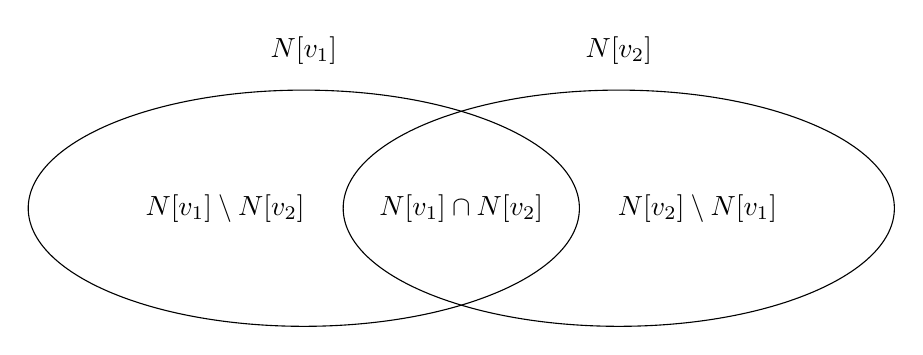
\begin{tikzpicture}
  \draw  (-2,1.5) ellipse (3.5 and 1.5);
  \draw  (2,1.5) ellipse (3.5 and 1.5);
  \node at (0,1.5) {$N[v_1] \cap N[v_2]$};
  \node at (-3,1.5) {$N[v_1] \setminus N[v_2]$};
  \node at (3,1.5) {$N[v_2] \setminus N[v_1]$};
  
  \node at (-2,3.5) {$N[v_1]$};
  \node at (2,3.5) {$N[v_2]$};
\end{tikzpicture}
\caption{$N[v_1]$ e $N[v_2]$, relação entre a vizinhança fechada de qualquer 2 vértices em um grafo de diâmetro 2}
\label{fig:setunion}
\end{figure}